% Fakesection 序言之前

\RequirePackage[l2tabu, orthodox]{nag}
\RequirePackage{ifxetex}
\RequireXeTeX
\documentclass{ctexart}

%颜色
\usepackage{xcolor}

%长度
\usepackage{printlen}
\uselengthunit{mm}

%图形
\usepackage{media9}
\usepackage{pdfpages}
\usepackage{overpic}
\usepackage{graphicx}
\graphicspath{{./src/}}
\usepackage{wallpaper}
\usepackage{wrapfig}
\usepackage{pstricks}
\usepackage{smartdiagram}
\usepackage[edges]{forest}
\usepackage{pgfplots}
\usepackage{tikz}
\usetikzlibrary{shapes.geometric}
\usetikzlibrary{calc}
\usetikzlibrary{patterns}
\usetikzlibrary{arrows}
\usetikzlibrary{shapes}
\usetikzlibrary{chains}
\usetikzlibrary{mindmap}
\usetikzlibrary{graphs}
\usepackage{scsnowman}
\usepackage{tikzpeople}
\usepackage{tikzducks}
\usepackage{pifont}
\usepackage{marvosym}
\usepackage{fontawesome}
\usepackage{stmaryrd}
\usepackage{ean13isbn}
\usepackage{qrcode}
\usepackage{pgf-pie}

%表格
\usepackage{tabu}
\usepackage{longtable}
\usepackage{booktabs}
\usepackage{diagbox}
\usepackage{multicol}
\usepackage{multirow}
\usepackage{makecell}
\usepackage{fancybox}
\usepackage{colortbl}
\usepackage{tcolorbox}
\tcbuselibrary{skins}
\tcbuselibrary{breakable}
\tcbuselibrary{theorems}
\tcbuselibrary{listings}
\tcbuselibrary{xparse}
\usepackage{fvextra}
\usepackage{csvsimple}
\usepackage{boxedminipage2e}

%公式
\usepackage{amsmath}
\usepackage{amsthm}
\usepackage{amsfonts}
\usepackage{amssymb}
\usepackage{amsbsy}
\usepackage{amsopn}
\usepackage{amstext}
\usepackage{mathrsfs}
\usepackage{bm}
\usepackage{textcomp}
\usepackage{latexsym}
\usepackage{exscale}
\usepackage{relsize}
%\usepackage{xymtex}
\usepackage{physics}
\usepackage{siunitx}
\usepackage{hologo}
\usepackage{cases}

%正文
\usepackage{fancyhdr}
\usepackage{geometry}
\usepackage{lastpage}
\usepackage{indentfirst}
\usepackage{setspace}
\renewcommand\arraystretch{1.5}

%非正文
\usepackage{makeidx}
\makeindex
\usepackage{epigraph}
\usepackage{varwidth}

%参考文献
\usepackage{morewrites}
\renewcommand{\thefootnote}{\fnsymbol{footnote}}
\usepackage[resetlabels]{multibib}
\newcites{sec}{参考网站}

%%链接
\usepackage
[	colorlinks = true,
linkcolor = gray,
citecolor = gray,
backref=page
]{hyperref}
\usepackage{caption}
\usepackage{subcaption}

%其它
\usepackage{atbegshi}
\usepackage{lipsum}

%文字
\usepackage{csquotes}
\usepackage{microtype}

\csname
endofdump
\endcsname

%\usepackage[notref,notcite]{showkeys}

%%代码
\usepackage{minted}
\tcbuselibrary{minted}% 用minted排版代码
%Java %与mcode冲突
% \usepackage{lstcustom}
%Matlab %与lstcustom冲突
%\usepackage[framed,numbered,autolinebreaks,useliterate]{mcode}
%\usepackage{boxie}
%\makeatletter
%\xdefinecolor{tcbcol@back}{rgb}{0,0,0}
%\makeatother

%枚举%与beamer冲突
\usepackage{enumitem}
\setlist[enumerate, 2]
{	fullwidth,
	label = \alph*.,
	font = \textup,
	itemindent=2em
}

\usepackage{titlesec}
%\titleformat{\chapter}{\centering\Huge\bfseries}{实验\chinese{chapter}~}{4mm}{}
\titleformat{\section}{\heiti\zihao{4}\bfseries}{\ifthenelse{\value{section}=0}{}{\thesection}~}{0pt}{\vspace{12pt}}[\vspace{12pt}]
\titleformat{\subsection}{\heiti\zihao{-4}\bfseries}{\arabic{section}.\arabic{subsection}~}{0pt}{\vspace{6pt}}[\vspace{6pt}]
\titleformat{\subsubsection}{\zihao{-4}}{ (\arabic{subsubsection}) ~}{0pt}{}
\titleformat{\paragraph}{\zihao{-4}}{第\chinese{paragraph},}{0pt}{}

\begin{document}

% Fakesection 评价页

\newgeometry{bottom=2cm}

\begin{titlepage}
	\centering
	\textbf{\fontsize{25pt}{\baselineskip}\kaishu{南京理工大学经济管理学院}}

	\vspace{5mm}
	\textbf{\fontsize{33pt}{\baselineskip}\lishu{课程论文}}

	\begin{table}[htpb]
		\centering
		\zihao{3}
		\begin{tabu}to.8\linewidth{@{}X[4,r]@{}X[c]@{}X[16,l]@{}}
			\makebox[4\ccwd][s]{课程名称}&:&\underline{\makebox[16\ccwd][c]{内部控制}}\\
			\makebox[4\ccwd][s]{论文题目}&:&\underline{\makebox[16\ccwd][c]{技术主导型企业内控问题探究分析}}\\
			\makebox[4\ccwd][s]{姓名}&:&\underline{\makebox[16\ccwd][c]{吴振宇}}\\
			\makebox[4\ccwd][s]{学号}&:&\underline{\makebox[16\ccwd][c]{916101630117}}\\
			\makebox[4\ccwd][s]{成绩}&:&\underline{\makebox[16\ccwd][c]{}}\\
			\makebox[4\ccwd][s]{任课教师评价}&~&
		\end{tabu}
		\zihao{-4}
		\begin{tabu}to.75\linewidth{@{}|X[l]|X[l]|@{}}
			\hline
			论文选题符合课程考核要求,具有一定的理论意义和实用价值,作者阅读较广泛,参考文献较充足。
			 &
			 \begin{tabu}{@{}X[l]@{}}
				 很好$ \square $ 较好$ \square $
				 \\
				 一般$ \square $ 尚可$ \square $
				 \\
				 差$ \square $
			 \end{tabu}
			 \\
			 \hline
			 论文观点正确,结构较合理,层次较清晰,逻辑性强,论述较全面,工作量较充实,结论具有一定的现实指导意义。
			 &
			 \begin{tabu}{@{}X[l]@{}}
				 很好$ \square $ 较好$ \square $
				 \\
				 一般$ \square $ 尚可$ \square $
				 \\
				 差$ \square $
			 \end{tabu}
			 \\
			 \hline
			 该生平时学习较认真,善于思考,到课率高,不迟到早退。文章语言表达较好,格
			 式符合规范要求,体现了较好的学风。
			 &
			 \begin{tabu}{@{}X[l]@{}}
				 很好$ \square $ 较好$ \square $
				 \\
				 一般$ \square $ 尚可$ \square $
				 \\
				 差$ \square $
			 \end{tabu}
			 \\
			 \hline
			 \begin{tabu}{@{}X[l]@{}}
				 教师签名:
				 \\
				 年~月~日
			 \end{tabu}
			 &
			 \\
			 \hline
		\end{tabu}
		\begin{flushleft}
			\makebox[5\ccwd][c]{}注:请将该封面与论文装订成册(论文双面打印)。
		\end{flushleft}
	\end{table}
\end{titlepage}

\restoregeometry

% Fakesection 摘要

\title{\heiti\zihao{2}\textbf{技术主导型企业内控问题探究分析}}
\author{\kaishu\zihao{4}\textbf{916101630117~吴振宇} }
\date{}
\maketitle

{
	\setlength{\baselineskip}{18pt}
	\kaishu

	\renewcommand{\abstractname}{}
	\begin{abstract}
		\zihao{5}
		\noindent
		\textbf{摘要: }随着我国社会经济的不断发展,市场竞争的日趋激烈,拥有核心技术、优良的创新环境、崇尚技术的企业文化的技术主导型企业越来越来被投资者和业内人士看好。然而在当今环境之下,部分企业盲目追崇技术而对企业的其他短板视之不见,从而招致企业衰败的事情也时有发生。如何在激烈的市场竞争中依靠技术的先进和制度的完善使企业长盛不衰已经成为了摆在现代企业面前的一项重大挑战。因此,从企业内部控制出发全面分析技术主导型企业的可能存在的各项问题尤为重要。本文基于明确属于技术主导型企业的一些企业的相关案例,层层剖析,并探讨了可行的解决方案。
	\end{abstract}

	\textbf{关键词:}技术主导型;内部控制;企业制度;问题与对策。

	\renewcommand{\abstractname}{}
	\begin{abstract}
		\zihao{5}
		\noindent
		\textbf{Abstract: }With the continuous development of China's social economy and the increasingly fierce market competition, technology-oriented enterprises with core technology, excellent innovation environment and technology-oriented corporate culture are increasingly favored by investors and industry insiders. However, in today's environment, some enterprises blindly adore technology while ignoring other shortcomings of enterprises, which leads to the decline of enterprises also occur from time to time. How to rely on the advanced technology and the improvement of the system in the fierce market competition to make the enterprise prosperous has become a major challenge for modern enterprises. Therefore, it is particularly important to comprehensively analyze the possible problems of technology-oriented enterprises from the perspective of internal control. Based on the relevant cases of some enterprises which belong to technology-oriented enterprises, this paper makes a layer-by-layer analysis and explores feasible solutions.
	\end{abstract}

	\textbf{Key Words: }Technology-oriented; Internal control; Enterprise system; Problems and countermeasures.

}

%页眉页脚%与book冲突
\pagestyle{fancy}
\renewcommand{\headrulewidth}{0pt}
\rhead{}
\lfoot{\small{\leftmark}}
\cfoot{\small{第\thepage 页~共~\pageref{LastPage}~页}}
\rfoot{\small{\rightmark}}

\setcounter{page}{1}

\section{引言}%
\label{sec:引言}

在当今技术爆炸的浪潮之下,一批企业文化崇尚技术、企业环境鼓励创新、拥有众多知识产权、以更新换代极快的高新技术产品为盈利点的企业通常被称为技术主导型企业。这类企业往往被众多投资者、业内人士看好,甚至忽视了这类企业一些其它的缺陷。但高新技术更新换代快,如果一时决策失败可能带来的结果就是企业由盛转衰,从昔日处于成长期的业内翘楚或成熟期的行业巨擎过早的进入衰败期。

因此,对技术主导型企业的内部制度,特别是内部控制环境暴露出的种种问题和现状进行分析,不仅具有理论上的价值,也具有一定的现实意义。本文就技术主导型企业内部控制存在的问题及需要采取的优化措施进行阐述。 \cite{陈国宏2012技术导向型产业集群创新研究——以沈阳高新区产业集群为例}

\begin{figure}[htpb]
	\centering
	\tikzset{
		planet/.append style={regular polygon, regular polygon sides=6},
		satellite/.append style={regular polygon, regular polygon sides=6},
		every picture/.append style={rotate=30},
		connection planet satellite/.style={
			bend right/.style=,
			every edge/.style={fill=\col},
			to path={
				\pgfextra
				\path[draw=none, fill=none] (\tikztostart)
				-- coordinate[at start] (@start@) coordinate[at end] (@target@) (\tikztotarget);
				\endpgfextra
				\ifnum\xi<\maxsmitem % to disable the last arrow
					($(@start@)!.6cm!90:(@target@)$) -- ($(@target@)!.25cm!-90:(@start@)$)
					-- ($(@target@)!.25cm!90:(@start@)$) -- ($(@start@)!.6cm!-90:(@target@)$)
					-- cycle
	\fi}}}
	\smartdiagram[connected constellation diagram]{
		企业\\生命\\周期,
		设立,
		发展,
		成长,
		成熟,
		衰退,
		倒闭
	}
	\caption{企业生命周期}
	\label{fig:企业生命周期}
\end{figure}

\section{技术主导型企业内控存在的问题}%
\label{sec:技术主导型企业内控存在的问题}

\subsection{唯技术论的企业文化忽视用户需求}%
\label{sub:唯技术论的企业文化忽视用户需求}

美国兰德公司 \footnote{ 美国兰德公司\href{https://www.rand.org/}{\faLink}是当今世界最负盛名的决策咨询机构。它先以研究军事尖端科学技术和重大军事战略而著称于世,继而又扩展到内外政策各方面,逐渐发展成为一个研究政治、军事、经济科技、社会等各方面的综合性战略研究机构。被誉为现代智囊的“大脑集中营”、“超级军事学院”以及世界智囊团的开创者和代言人。} 把企业竞争力分为3个层面:产品层、制度层和文化层。

\begin{description}
	\item[产品层:]表层的竞争力;
	\item[制度层:]支撑平台的竞争力;
	\item[文化层:]最基础、最核心的竞争力,即企业的信念和价值观。诸如企业文化、企业价值理念等深层次的东西却是很难模仿和复制的。
\end{description}

\begin{figure}[htpb]
	\centering
	\smartdiagramset{
		set color list={blue!50!cyan,green!60!lime,orange!50!red},
		priority arrow width=2cm,
		priority arrow height advance=2.25cm
	}
	\smartdiagram[priority descriptive diagram]{产品层,制度层,文化层}
	\caption{企业竞争力}
	\label{fig:企业竞争力}
\end{figure}

企业文化对公司的发展导向作用是毋庸置疑的。技术主导型企业文化对于企业能够通过知识资源的开发利用获得企业核心竞争力意义重大。企业如果没有很好的人才储备和较强的学习能力,仅仅通过从外部购买技术,是难于从产品质量中获得竞争优势的;虽然技术主导型企业前期发展比较慢,但是,越往后发展越快,因为它的核心竞争力是技术,而技术转化为生产力往往需要一个漫长的过程。

然而如果企业过于重视技术走向 \enquote{唯技术论}的误区,则会因忽视用户需求做出那些技术含量极高但却与市场严重脱轨而无人问津的产品。在产品更新换代频繁的高新技术产业,一个产品研发方向的错误往往就会导致一个公司的重大损失。

一个最典型的例子就是摩托罗拉著名的铱星计划。 \cite{吴定祥2015中国联想并购摩托罗拉案例分析} 摩托罗拉是一个很重视产品规划的公司,此前摩托罗拉每开发一款新产品,通常先提前数月预测消费趋势。但在快速升级换代的手机行业中,制造商们试图提前数月预测消费者需求是非常困难的。再加上摩托罗拉是一家技术主导型的公司,工程师文化非常浓厚,这种公司通常以自我为中心,唯“技术论” ,从而导致摩托罗拉虽然有市场部门专门负责收集消费者需求的信息,但在技术主导型的企业文化里,消费者的需求很难被研发部门真正倾听,研发部门更愿意花费大量精力在那些复杂系统的开发上,从而导致研发与市场需求的脱节。

\begin{figure}[htpb]
	\centering
	\begin{subfigure}[htpb]{.45\linewidth}
		\centering
		
\includegraphics[width=\linewidth]{motorola.jpg}
		\caption{摩托罗拉徽标}
		\label{fig:摩托罗拉徽标}
	\end{subfigure}
	\quad
	\begin{subfigure}[htpb]{.3\linewidth}
		\centering
		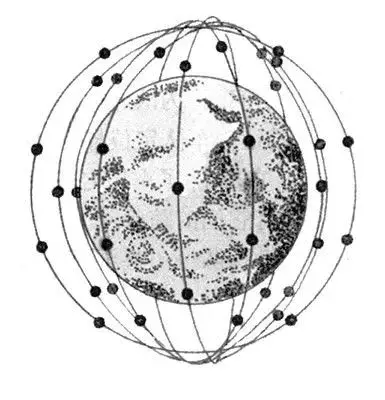
\includegraphics[width=\linewidth]{77.png}
		\caption{铱星计划}
		\label{fig:铱星计划}
	\end{subfigure}
	\caption{摩托罗拉与铱星计划}
	\label{fig:摩托罗拉与铱星计划}
\end{figure}

为了夺得对世界移动通信市场的主动权,并实现在世界任何地方使用无线手机通信,以摩托罗拉为首的美国一些公司在政府的帮助下,于 1987 年提出新一代卫星移动通信星座系统——铱星。 \cite{罗慧辉2005技术创新与市场的碰撞———“铱星计划”与“小灵通”的案例比较研究}

铱星系统技术上的先进性在目前的卫星通信系统中处于领先地位。铱星系统卫星之间可通过星际链路直接传送信息,这使得铱星系统用户可以不依赖地面网而直接通信,但这也恰恰造成了系统风险大、成本过高、维护成本相对于地面也高出许多。整个卫星系统的维护费一年就需几亿美元之巨。

铱星的高科技含量举世公认,但铱星手机价格每部高达 3000 美元,加上高昂的通话费用,它开业的前两个季度,在全球只发展了 1 万用户,这使得铱星公司前两个季度的亏损即达 10 亿美元。尽管铱星手机后来降低了收费,但仍未能扭转颓势。

\subsection{治理结构的混乱导致了对衰败苗头的视而不见}%
\label{sub:治理结构的混乱导致了对衰败苗头的视而不见}

早在 2008 年 5 月,市场调研厂商 IDC 和战略分析公司Strategy Analytics 表示,摩托罗拉可能在 2008 年底之前失去北美市场占有率第一的位置。摩托罗拉的当季报也显示,2008 年第一季度全球手机销量下降 39\%, 手机部门亏损 4.18亿美元,与上年同期相比亏损额增加了 80\%。

\begin{figure}[htpb]
	\centering
	\begin{tikzpicture}
		\begin{axis}[ybar,enlargelimits=0.15]  % 绘制关于y坐标的条形图,条形之间的最大间隔是0.15cm
			\addplot[draw=blue,fill=red]           % 蓝色边界、红色填充
				coordinates
				{
					(1,99.93) (2,94.09) (3,89.63) (4,88.81)
				};
			\addplot[draw=black,fill=blue]         % 黑色边界、蓝色填充
				coordinates
				{
					(1,110.83) (2, 106.85) (3, 103.58) (4, 103.73)
				};
			\addlegendentry{资产/负债 (亿) };
		\end{axis}
	\end{tikzpicture}
	\caption{各季度资产/负债}
	\label{fig:各季度资产/负债}
\end{figure}

根据资产负债表\ref{tab:摩托罗拉资产负债表},可见负债的规模正在逐年增长,负债方面存在着比较大的上升\%。企业负债规模会影响企业的发展,显而易见,企业负债规模过大,就会产生企业利息支出增大的问题,企业的收益也会相应的减少,偿付能力就会减弱,使得筹资风险增大。在企业的总负债当中,由于长期和短期负债占比不可能完全相同,缺乏合理安排长期负债的比例,增加了企业融资的风险。资产规模也在逐年增长,企业偿还债务的能力逐年减弱,存在一定的财务风险。

而在问题出现的时候,管理层在做什么呢?注意这时已经过去20年,铱星计划的失败已经非常明显,而摩托罗拉公司内部仍然在产品的定位、公司的福利等事上纠缠不清:公司不考虑手机的细分发展,3年时间仅依赖V3一个机型。没有人会否认V3作为一款经典手机的地位,正是依靠V3,摩托罗拉2005年全年利润提高了102\%,手机发货量增长40\%,摩托罗拉品牌也重焕生机。尽管V3让摩托罗拉重新复苏,更让摩托罗拉看到了夺回市场老大的希望。然而,摩托罗拉过分陶醉于V3带来的市场成功。赛迪顾问研究显示,2005年以前是明星机型的天下,一款明星手机平均可以畅销2-3年,而过了2005年,手机市场已成了细分市场的天下,手机行业已经朝着智能化、专业拍照、娱乐等方向极度细分,而摩托罗拉似乎对此视而不见。在中国市场,2007年摩托罗拉仅仅推出13款新机型,而其竞争对手三星推出了54款机型,诺基亚也有37款。——价格跳水快,自毁品牌形象。在新品跟不上的情况下,降价成了摩托罗拉提高销量不得不采取的手段。许多摩托罗拉的忠实用户把摩托罗拉的手机称为“(价格)跳水冠军”。以V3为例,从刚上市时的6000多元的高端时尚机型跌入4000多元的白领消费群,再到2000多元的普通时尚消费群,直到停产前的1200多元。短期的大幅降价让不少高端用户无法接受,同时也对V3的定位产生了质疑,后果就是对摩托罗拉品牌彻底失去信任。而当外部环境使得摩托罗拉进入战略收缩期,赢利空间不再,摩托罗拉公司依旧维持着高福利的企业传统。

管理层对各种问题视而不见和重大决策上的频频失误,对公司的衰败有着不可推卸的责任。摩托罗拉资深副总裁吉尔莫曾说: \enquote{摩托罗拉内部有一种亟须改变的‘孤岛传统’。}

\subsection{风险评估和预算控制的失策}%
\label{sub:风险评估和预算控制的失策}

在制定各种战略投资之前进行风险评估和预算控制是一个企业能否成功趋利避害,在风险和收益之间寻求一个可靠的平衡的重要因素。

还是以铱星计划为例,该系统风险大、成本过高、维护成本相对于地面也高出许多。整个卫星系统的维护费一年就需几亿美元之巨。高技术带来的高风险即使是摩托罗拉这样的大公司也无法承受,预算的不足更是雪上加霜。除了摩托罗拉等公司提供的投资和发行股票筹集的资金,铱星计划举借的债务高达30亿美元,每月光债务利息就达4000多万美元。甚至当这个项目破产时仍然有40亿美元的债务无法偿还。

摩托罗拉在债务面前为了尽快盈利,让铱星系统在在系统本身不完善的情况下投入商业服务的决定是“毁灭性的”。匆匆投入商用的铱星计划的低质服务给用户留下的第一印象对于铱星公司来说是灾难性的。用户普遍反映铱星手机通信不稳定。因此,这种形象严重阻碍了其市场拓展和巩固。到2000年3月铱星公司宣布破产保护时为止,铱星公司的客户还只有两万多家。 \cite{郭国庆2000技术创新与市场营销──美国铱星公司和}

\begin{figure}[htpb]
	\centering
	\begin{tikzpicture}
		\pie[pos={0,0},radius=2,rotate=0]{3.3/铱星系统用户,96.7/地面蜂窝系统用户}
	\end{tikzpicture}
	\caption{铱星系统和地面蜂窝系统用户比}
	\label{fig:铱星系统和地面蜂窝系统用户比}
\end{figure}

\section{总结}%
\label{sec:总结}

创建和谐的企业内部控制环境,关乎企业的盛衰荣辱和生死存亡。企业的内部控制环境是内部控制的关键,确定了一个企业的基调,它影响着整个企业内部所有人员的控制意识。

根据分析结果,可以得到以下结论:

\begin{description}
	\item[工程师精神的企业文化要避免走向唯技术论的极端]摩托罗拉的企业文化崇尚技术和创新。当初工程师巴里·伯蒂格因为妻子在加勒比海度假时说她无法用手机联系到她的客户的一句抱怨而产生的突发奇想,得到了当时任公司董事长的加尔文决心把这一计划付诸实践的支持。可见该公司对创新的支持力度之大。然而铱星计划的失败不是技术的失败,只论技术不论市场的盲目乐观早已注定了铱星计划要失败。
	\item[建立完善的组织结构]铱星公司的基本市场运行组织结构是一个由世界上多个辖管地区性 \enquote{闸口} 国家或企业组成的合伙人结构。由于各地区\enquote{闸口}仅负责在本地区范围内的铱星卫星移动通信系统的手持电话的销售和提供相应的服务,各自的利益关系和产权关系极不清晰,导致铱星计划根本无法建立一个面向全球性的市场运营构架。 \cite{杨有红2004试论公司治理与内部控制的对接}
	\item[正确使用各种内控手段进行调节]之前的分析已经表明摩托罗拉公司的风险评估和预算控制存在严重失策,像风险分析上的盲目乐观,认为用户都属于“付钱不看账单的一群人”的高层次的国际商务旅行人员。对预算的错误估计导致在系统还未完善的时候就不得不急于推出,而糟糕的用户体验又进一步为之后的失败奠定了祸根。
\end{description}

综上,技术主导型企业更应该加强内控环境的完善,正确应用各项内控手段进行,才能最大程度避免风险,赢得预期的收益。

% Fakesection 参考文献

\bibliographystyle{IEEEtran}
\bibliography{src/main}

% Fakesection 附录

\appendix

\section{数据}%
\label{sec:数据}

\begin{table}[htpb]
	\centering
	\caption{摩托罗拉资产负债表}
	\label{tab:摩托罗拉资产负债表}
\end{table}
\csvautobooklongtable{src/motorola.csv}

\end{document}

